\section{Experimental Results and Interpretation}
\label{sec:results}
\subsection{Effect of the library implementation}
Table~\ref{tab:impl} summarizes AES-128-CTR throughput at 32 MiB. On Windows, the OpenSSL transform rate is 5537 MB/s, compared with 2877 MB/s for PyCryptodome. On Arm64, default OpenSSL reaches 4030 MB/s, whereas the masked OpenSSL configuration and PyCryptodome achieve 218 and 209 MB/s, respectively. These values are medians across five sessions for each configuration.

\begin{table}[htbp]\centering\caption{AES-128-CTR, 32 MiB: throughput by platform, implementation and timing scope (decimal MB/s).}\label{tab:impl}\small
\begin{tabular}{llrr}\toprule
Host & Implementation & Transform & Full call\\\midrule
Windows i5-10300H & OpenSSL EVP & 5537 & 1479\\
Windows i5-10300H & PyCryptodome & 2877 & 1202\\
Oracle Arm64 & OpenSSL default & 4030 & ---\\
Oracle Arm64 & OpenSSL armcap=0 & 218 & ---\\
Oracle Arm64 & PyCryptodome & 209 & ---\\\bottomrule\end{tabular}
\par\smallskip\parbox{\linewidth}{\footnotesize Transform and full-call rates use the intervals defined in Section~\ref{sec:method}. Full call denotes the instrumented operation. Dashes indicate results outside the Arm64 transform dataset analyzed here.}
\end{table}

The Arm64 difference is large and repeatable within the recorded sessions. The default OpenSSL session medians range from 4018 to 4035 MB/s, while the masked configuration ranges from 217.4 to 218.4 MB/s and PyCryptodome from 208.8 to 209.5 MB/s. The approximately 19-fold throughput ratio between default OpenSSL and PyCryptodome therefore reflects a persistent difference between the evaluated paths. The reduction under capability masking also shows that OpenSSL's optimized capability selection is important on this host. Because the mask disables several features, the result cannot be attributed exclusively to AES instructions.

Figure~\ref{fig:size} places the 32 MiB results in the context of message size. Larger payloads sustain substantially higher OpenSSL throughput than the alternative paths on each host. At 1 KiB, the native transform interval is very short, making the calculated rate more sensitive to timer resolution and call overhead. Large-buffer throughput should consequently not be used to predict the latency of short requests. The two panels describe separate software environments; differences between them are not estimates of an intrinsic x86-64 versus Arm64 performance ratio.

\begin{figure}[htbp]\centering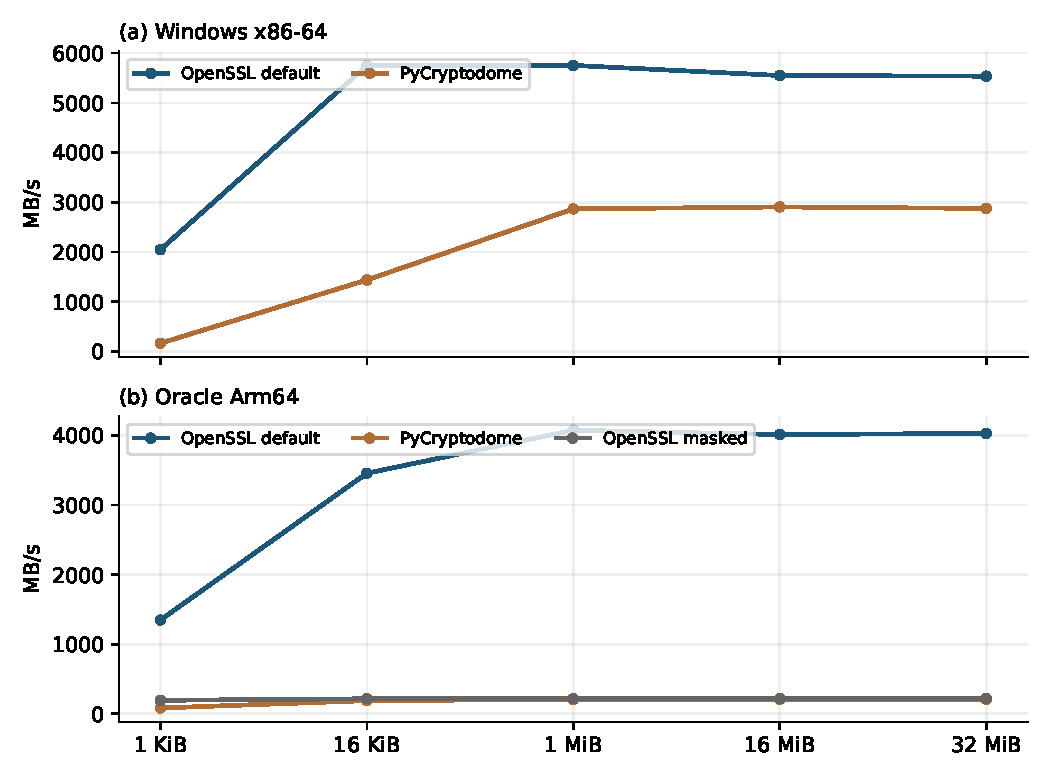
\includegraphics[width=.96\linewidth]{figures/ctr_size_curves.pdf}
\caption{AES-128-CTR transform throughput versus payload size on (a) Windows x86-64 and (b) Oracle Arm64. Each panel compares implementations within one host.}\label{fig:size}\end{figure}

\subsection{Effect of the timed software operation}
Expanding the Windows timer from transformation to the instrumented operation changes the magnitude of the library difference (Fig.~\ref{fig:windows}). OpenSSL throughput decreases from 5537 to 1479 MB/s, while PyCryptodome decreases from 2877 to 1202 MB/s. The ratio of their aggregate rates consequently falls from approximately 1.93 to 1.23. Across sessions, the broader OpenSSL rate ranges from 1452 to 1625 MB/s and the PyCryptodome rate from 1179 to 1263 MB/s.

\begin{figure}[htbp]\centering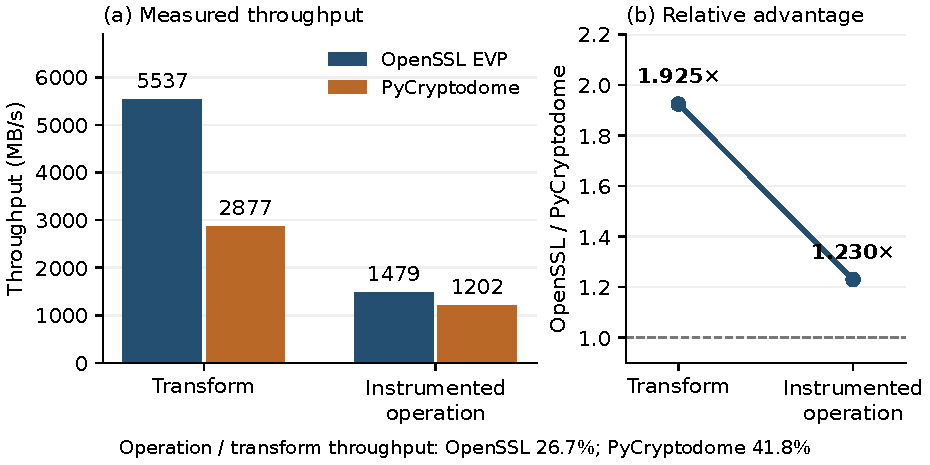
\includegraphics[width=.88\linewidth]{figures/windows_boundaries.pdf}
\caption{AES-128-CTR throughput at 32 MiB on Windows: transform processing and the instrumented operation. The broader interval includes preparation, result handling and benchmark diagnostics.}\label{fig:windows}\end{figure}

The ordering remains the same, but the advantage is smaller when additional work is timed. Selecting the faster cipher path therefore does not produce an equally large improvement at every surrounding interface. Allocation, bindings, setup, result conversion and instrumentation contribute to the broader measurement, with different costs in each implementation. The measurements do not isolate their individual contributions, and subtracting aggregate medians would not provide a valid cost decomposition.

For application design, the relevant implication is to measure the interface actually used by the service. The instrumented operation demonstrates the sensitivity to measurement scope, but its diagnostic overhead prevents treating 1479 or 1202 MB/s as a prediction of production throughput. Buffer reuse, persistent contexts and different language bindings could change the relationship and require separate evaluation.

\subsection{Key length and authenticated processing}
The separate CBC experiment shows how key length affects both absolute throughput and relative acceleration (Table~\ref{tab:cbc}). Software encryption decreases from 225.1 MB/s for AES-128 to 174.9 MB/s for AES-256; the AES-NI path decreases from 531.6 to 474.0 MB/s. Nevertheless, the session-based acceleration factor increases from 2.37 to 2.71. Thus, a larger relative benefit from acceleration can coexist with lower absolute throughput. The pattern is consistent with the additional rounds required by longer keys, although the measured factors remain specific to this implementation and mode.

\begin{table}[htbp]\centering\caption{AES-CBC encryption at 10 MiB on Windows (MB/s). Speedups are medians of session-level time ratios.}\label{tab:cbc}
\begin{tabular}{lrrr}\toprule Key length & Software & AES-NI path & Speedup\\\midrule
AES-128 & 225.1 & 531.6 & 2.37$\times$\\
AES-192 & 198.5 & 504.3 & 2.53$\times$\\
AES-256 & 174.9 & 474.0 & 2.71$\times$\\\bottomrule\end{tabular}\end{table}

Authenticated processing introduces a different workload. Table~\ref{tab:gcm} reports representative GCM sizes, and Fig.~\ref{fig:gcm} includes all five evaluated sizes. At 1 KiB, AES-128 encryption reaches 70.6 MB/s, while verified decryption reaches 38.1 MB/s. At 1 MiB, the corresponding rates rise to 1148.2 and 1131.4 MB/s. The encryption--decryption difference is therefore much more pronounced for short messages than for large buffers.

\begin{table}[htbp]\centering\caption{AES-GCM payload throughput on Windows (MB/s). Encryption includes tag generation; decryption includes verification. Cipher-object construction is excluded.}\label{tab:gcm}\small
\begin{tabular}{llrr}\toprule Payload & Variant & Encrypt & Verify/decrypt\\\midrule
1 KiB & AES-128-GCM & 70.6 & 38.1\\
1 KiB & AES-256-GCM & 70.1 & 38.0\\
1 MiB & AES-128-GCM & 1148.2 & 1131.4\\
1 MiB & AES-256-GCM & 1059.3 & 1059.8\\
100 MiB & AES-128-GCM & 1179.7 & 1189.3\\
100 MiB & AES-256-GCM & 1100.4 & 1080.4\\\bottomrule\end{tabular}\end{table}

\begin{figure}[htbp]\centering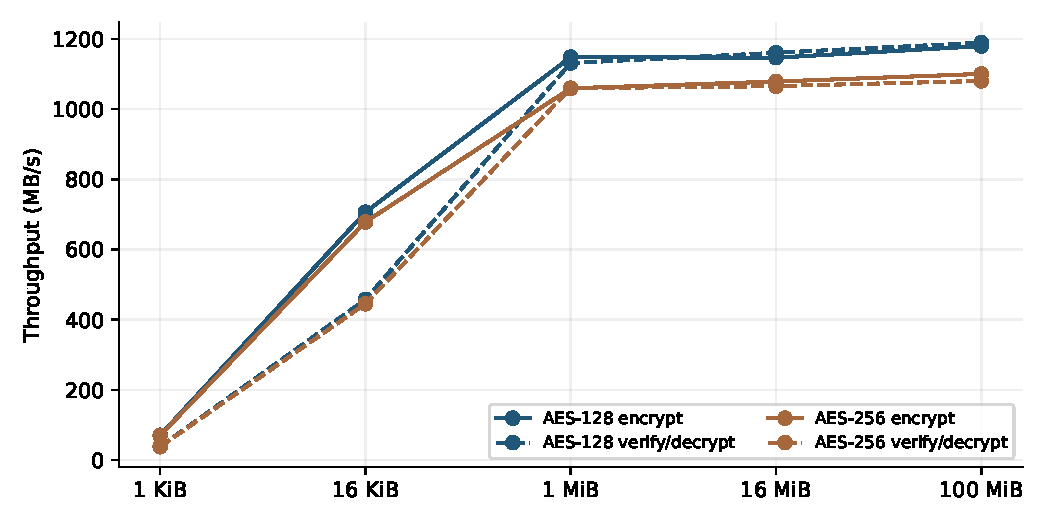
\includegraphics[width=.88\linewidth]{figures/gcm_payload_size.pdf}
\caption{AES-GCM encryption and verified-decryption throughput on Windows for five payload sizes. Lines connect the measured aggregate rates.}\label{fig:gcm}\end{figure}

This pattern is consistent with fixed processing costs being distributed over more payload bytes as message size increases. The plateau at larger sizes suggests that additional payload then increases processing time approximately in proportion to its length over the measured range. AES-256 generally achieves lower throughput than AES-128, as expected from its additional rounds. However, the experiment does not separately time authentication multiplication, verification or allocation, so it cannot assign the observed size dependence to one component.

These GCM results complement the CTR and CBC observations by showing why a benchmark must represent the required cryptographic service. GCM includes authentication, whereas the CTR and CBC workloads reported here measure confidentiality operations. Their throughput figures therefore describe different functionality. The GCM timer also excludes object construction, so a service handling independent messages must additionally account for setup and its surrounding request-processing costs.
